\section{Wprowadzenie}

Bardzo ważnym etapem analizy wyników jest ich merytoryczna ocena. Z punktu widzenia przeprowadzonego badania, cenny byłby dostęp do danych pochodzących ze źródeł podatkowych --- w celu porównania np. rozkładów dochodu w populacji. 

Pierwsza część rozdziału zawiera porównanie oszacowań pośrednich wskaźników ubóstwa z~danymi z rejestrów administracyjnych. Z uwagi na brak dostępu do odpowiednio szczegółowych danych dotyczących ubóstwa, w celu przeprowadzenia merytorycznej oceny zaproponowano użycie \textit{zmiennych proxy} pochodzących z Banku Danych Lokalnych.

W drugiej części rozdziału zaproponowano zastosowanie miary odległości w ocenie oszacowań pośrednich wskaźników ubóstwa. Na podstawie odległości euklidesowej oraz uogólnionej miary odległości \citep{walesiak2011} utworzono ranking podregionów i powiatów oraz dokonano porównania otrzymanych wyników z rankingiem utworzonym w oparciu o wartości wskaźników ubóstwa. 

W rozdziale przeprowadzono także przestrzenną analizę ubóstwa w Polsce. Otrzymane rezultaty przedstawiono na kartogramach, które pozwalają na analizę przestrzennych zależności \citep{simler2007}. Dokonano także grupowania wartości stopy i głębokości ubóstwa metodą k-średnich, w celu utworzenia homogenicznych klas zawierających zbliżone wartości. Na tej podstawie zidentyfikowano obszary najmniej i najbardziej narażone na występowanie zjawiska ubóstwa. Ponadto przeprowadzono ocenę spójności przestrzennej oszacowań pośrednich wskaźników ubóstwa z wykorzystaniem statystyki Morana I. 

\section{Zbieżność wyników estymacji pośredniej z danymi z rejestrów}

W sytuacji, w której nie są znane wartości wskaźników ubóstwa w populacji można posłużyć się tzw. \textit{zmiennymi proxy} \citep{analpovdata42016}. Wybór tych cech powinien być uzasadniony i~musi występować związek pomiędzy analizowaną cechą, a \textit{zmienną proxy}. Osoby, które korzystają ze świadczeń pomocy społecznej (zmienna proxy) są ubogie (zmienna analizowana). To samo można zauważyć w stosunku do osób, które otrzymują zasiłek dla bezrobotnych. Odsetek osób otrzymujących świadczenie stanowi zmienną proxy dla liczby osób bezrobotnych. Trzeba jednak zauważyć, że nie zachodzi relacja odwrotna --- nie wszystkie osoby bezrobotne otrzymują zasiłek \citep{fenton2013}. 

Oszacowania stopy oraz głębokości ubóstwa porównano z danymi dotyczącymi bezrobocia rejestrowanego oraz korzystania z pomocy społecznej. Wykorzystane zmienne pochodziły z rejestrów, a zatem nie były obciążone błędem losowym przez co można je uznać ze precyzyjne miary porównawcze. Ponadto są to cechy ściśle związane ze zjawiskiem ubóstwa \citep{jakosc-gus2017}. Z zakresu bezrobocia rejestrowanego pod uwagę brano dwie cechy (w nawiasach podano skrótowe nazwy wykorzystywane na rysunkach):

\begin{itemize}
\item udział osób bezrobotnych zarejestrowanych pozostających bez pracy dłużej niż 1 rok w~liczbie bezrobotnych ogółem (Ods. bezr. 12m),
\item udział osób bezrobotnych zarejestrowanych pozostających bez pracy dłużej niż 1 rok w~liczbie osób aktywnych zawodowo (Stopa bezr. 12m).
\end{itemize}

Z kolei z zakresu pomocy społecznej wybrano zmienne, które mogą być miernikiem ubóstwa:

\begin{itemize}
\item zasięg korzystania ze środowiskowej pomocy społecznej ogółem (Zasięg PS ogół.),
\item zasięg korzystania ze środowiskowej pomocy społecznej wśród osób poniżej kryterium dochodowego (Zasięg PS doch.).
\end{itemize}

Należy jednak zwrócić uwagę na to, że zasięg korzystania ze środowiskowej pomocy społecznej to odsetek osób, które muszą spełniać dwa kryteria: kwalifikować się do otrzymania takiej pomocy oraz zgłosić się do odpowiedniej placówki w obrębie gminy.

\subsection{Poziom podregionów}\label{pr:mer-podreg}

W pierwszej kolejności dokonano oceny oszacowań uzyskanych na poziomie podregionu. Zestawiono ze sobą bezpośrednie oszacowania stopy oraz głębokości ubóstwa, szacunki pośrednie oraz wartości \textit{zmiennych proxy} pochodzące z rejestrów administracyjnych.

\begin{figure}[ht]
\caption{Porównanie oszacowań stopy ubóstwa z danymi pochodzącymi z rejestrów administracyjnych na poziomie podregionów}
\centering
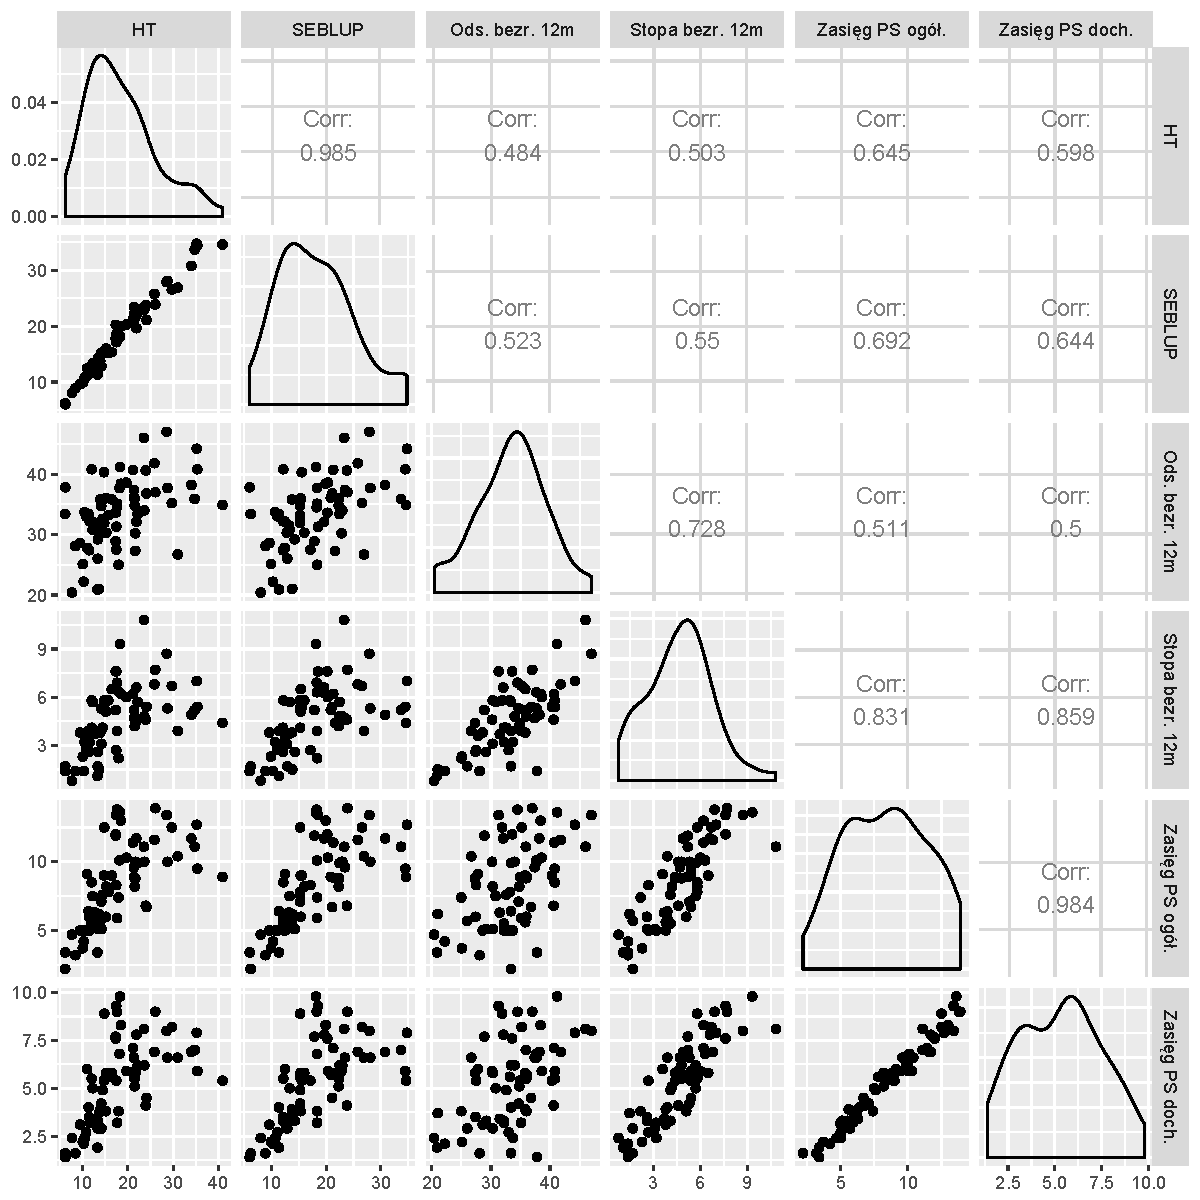
\includegraphics[width=0.8\textwidth]{05_wykresy/hcr_podreg_por-1.pdf}\\
\small{Źródło: opracowanie własne na podstawie EU-SILC 2011 oraz BDL.}
\label{fig:hcr_podreg_por}
\end{figure}

Na podstawie danych zawartych na rysunku \ref{fig:hcr_podreg_por} można zaobserwować, że oszacowania bezpośrednie i pośrednie są do siebie bardzo zbliżone. Oszacowania bezpośrednie są najsilniej skorelowane z zasięgiem korzystania ze środowiskowej pomocy społecznej ogółem ($r=0,645$). Podobnie jest w przypadku oszacowań pośrednich --- odnotowano nieznaczny wzrost wartości współczynnika korelacji do poziomu $r=0,692$. Stopa ubóstwa ekonomicznego wyznaczona z zastosowaniem estymatora SEBLUP jest przeciętnie 2,2 razy wyższa od zasięgu korzystania z pomocy społecznej. W obliczeniach przyjęto granicę ubóstwa równą 60\% mediany dochodów ekwiwalentnych, która w 2011 roku była dwukrotnie wyższa od granicy ustawowej (por. podrozdział \ref{pr:czasowy-wymiar-ubostwa}). Zależność pomiędzy stopą ubóstwa, a długotrwałym bezrobociem ma charakter umiarkowany. Wysoka korelacja istnieje także pomiędzy stopą bezrobocia długotrwałego i zasięgiem korzystania z pomocy społecznej. Należy jednak zwrócić uwagę na fakt, że współczynniki korelacji dla oszacowań pośrednich są zawsze wyższe od poziomu tych współczynników dla estymacji bezpośredniej \citep{wawrowski2016}.

W przypadku głębokości ubóstwa dokonano analogicznego porównania. W otrzymanych wynikach zaobserwowano identyczne zależności, co w przypadku stopy ubóstwa, z tą różnicą, że wartości współczynników korelacji były mniejsze. Wynika to z faktu, że głębokość ubóstwa mierzy bardzo specyficzne zjawisko (ubóstwo osób ubogich), które jest trudne w obserwacji na poziomie wskaźników społecznych. Odpowiednie korelogramy znajdują się w załączniku.

\subsection{Poziom powiatów}

Podobnie, jak w przypadku podregionów (por. \ref{pr:mer-podreg}) porównania oszacowań wskaźników ubóstwa dokonano na poziomie powiatów. W tym przypadku oszacowania pośrednie będą reprezentowane przez trzy estymatory: SEBLUP obliczony na poziomie obszaru oraz EB i MQ wykorzystujące dane jednostkowe. Wyniki porównania przedstawione są na rysunku \ref{fig:hcr_pow_por}.

\begin{figure}[ht]
\caption{Porównanie oszacowań stopy ubóstwa z danymi pochodzącymi z rejestrów administracyjnych na poziomie powiatów}
\centering
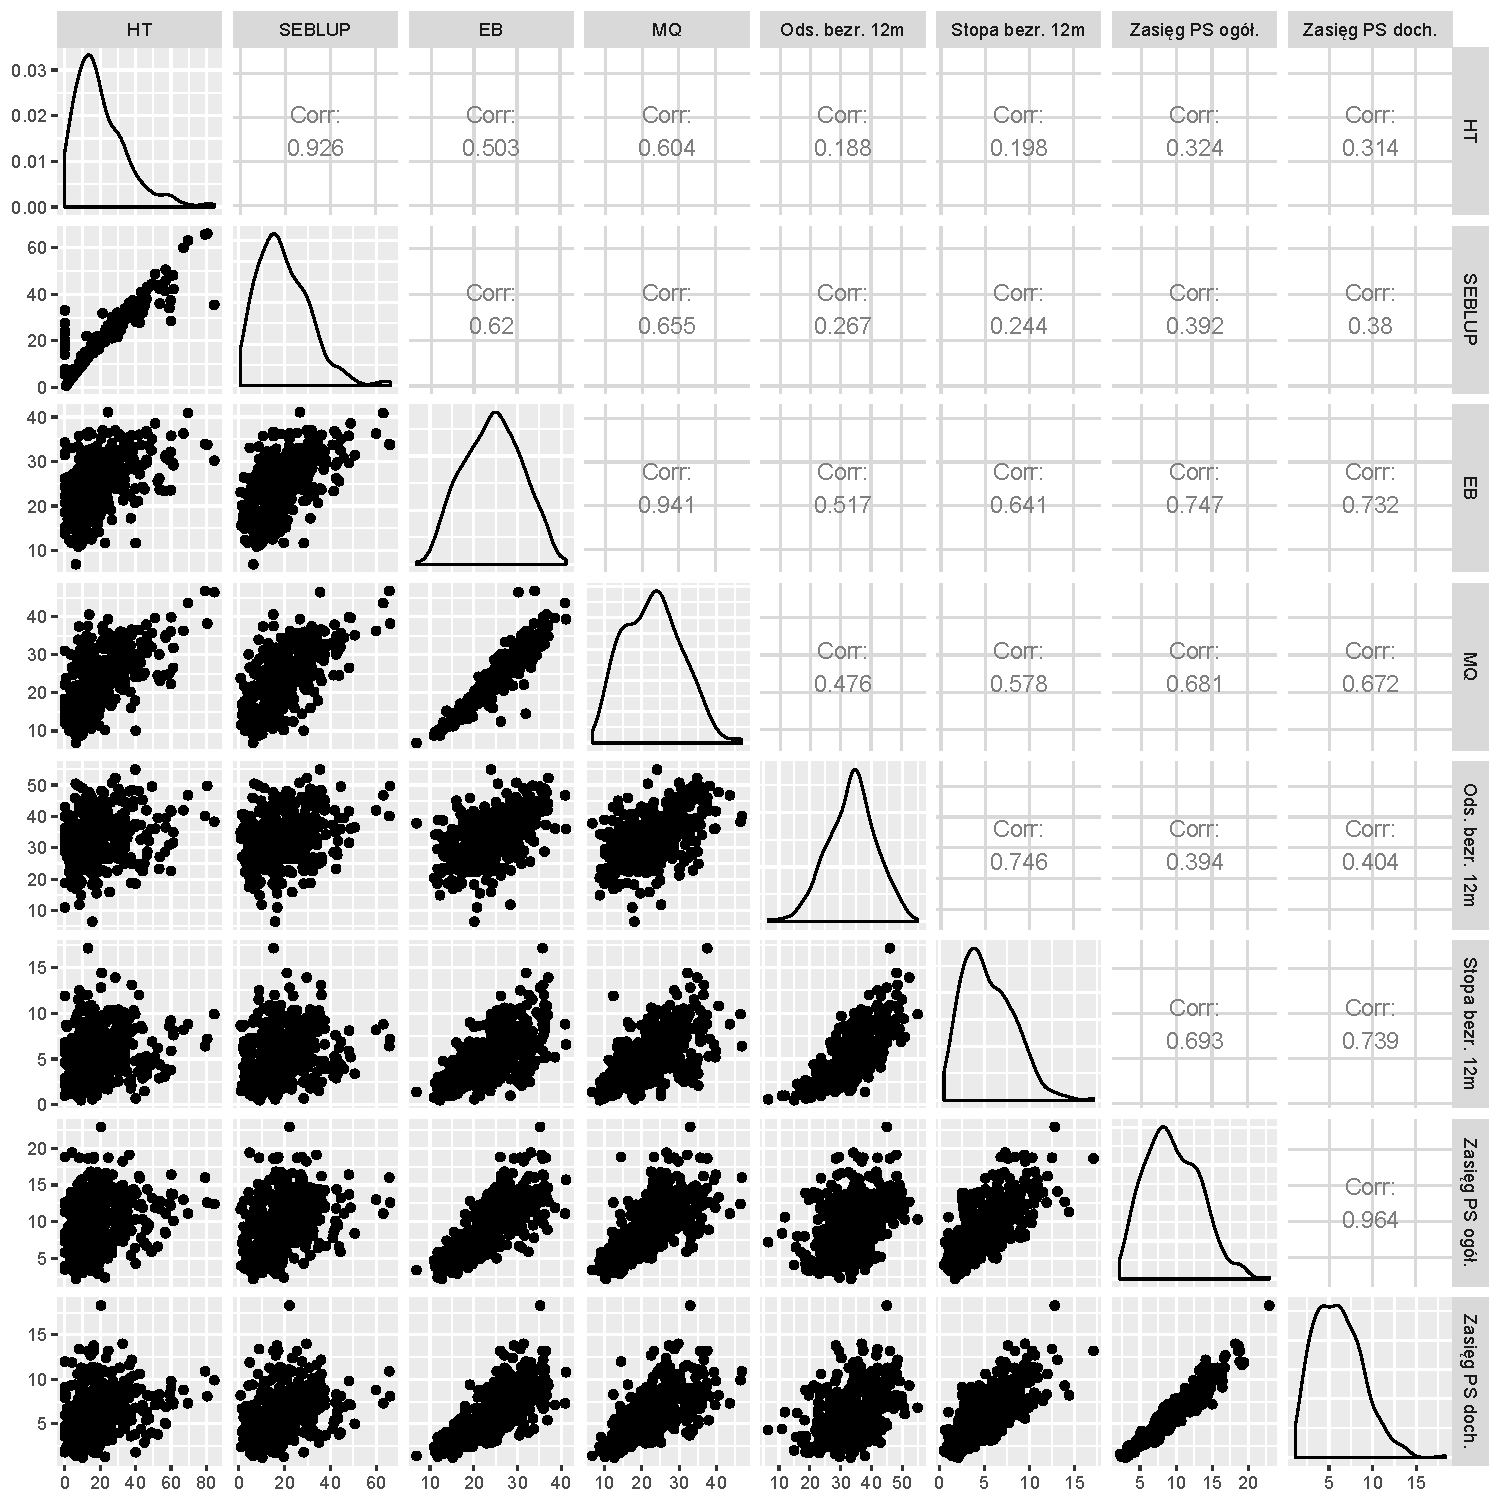
\includegraphics[width=0.8\textwidth]{05_wykresy/hcr_pow_por-1.pdf}\\
\small{Źródło: opracowanie własne na podstawie EU-SILC 2011, NSP 2011 oraz BDL.}
\label{fig:hcr_pow_por}
\end{figure}

Otrzymane zestawienie pokazuje, że oszacowania bezpośrednie są w bardzo małym stopniu skorelowane ze wskaźnikami z zakresu bezrobocia ($r=0,198$) i pomocy społecznej ($r=0,324$). Zastosowanie podejścia obszarowego w postaci estymatora SEBLUP przyczynia się do zwiększenia podobieństwa pomiędzy wartościami stopy ubóstwa oraz zmienną zasięg korzystania z~pomocy społecznej. Niemniej ta zmiana nie jest istotna (o 0,068) i nie przyczynia się do zmiany rodzaju zależności --- jest to wciąż korelacja słaba. Istotną poprawę widać natomiast w przypadku zastosowania podejścia jednostkowego --- estymatorów EB i MQ. Oszacowania otrzymane z wykorzystaniem obydwu metod są do siebie bardzo zbliżone, współczynnik korelacji liniowej Pearsona wynosi 0,941. Porównanie tych oszacowań ze stopą bezrobocia długotrwałego pokazuje istotny wzrost wartości w porównaniu do estymacji bezpośredniej. W przypadku metody EB $r=0,641$, a w przypadku metody M-kwantylowej współczynnik korelacji wynosi 0,578. Najwyższe wartości współczynników obserwuje się dla cechy: zasięg korzystania ze środowiskowej pomocy społecznej ogółem. W tym przypadku korelacja jest silna i wynosi $r=0,747$ (estymator EB) oraz $r=0,681$ (estymator MQ). Także na poziomie powiatów obserwowana jest zależność wskazująca, że pośrednie oszacowania stopy ubóstwa są średnio 2,2 razy wyższe od zasięgu korzystania z pomocy społecznej ogółem. Wartości współczynników korelacji otrzymane dla wskaźnika głębokości ubóstwa były bardzo podobne do tych, które otrzymano dla stopy ubóstwa (por. Załącznik).

Wyniki estymacji wskazują zatem, że oszacowania pośrednie uzyskane z wykorzystaniem podejścia obszarowego na poziomie podregionów oraz oszacowane na podstawie podejścia jednostkowego na poziomie powiatów w dużo większym stopniu są zbieżne z rzeczywistymi wartościami aniżeli oszacowania bezpośrednie. Większe podobieństwo pomiędzy oszacowaniami i wskaźnikami pochodzącymi z rejestrów administracyjnych stanowi argument przemawiający za stosowaniem metod statystyki małych obszarów.

\section{Wielowymiarowa analiza statystyczna poziomu ubóstwa}

W ocenie poziomu ubóstwa można także wykorzystać metody wielowymiarowej analizy statystycznej. Na podstawie oszacowań wskaźników ubóstwa uzyskanych z zastosowaniem metod estymacji pośredniej można utworzyć ranking jednostek terytorialnych --- od najmniej zagrożonych niedostatkiem do tych najbardziej narażonych na występowanie tego zjawiska. Tak uporządkowane jednostki można porównać z rankingiem podregionów czy powiatów otrzymanym na podstawie syntetycznego miernika rozwoju, który uwzględnia cechy ekonomiczno-demograficzne związane z~opisywanym zjawiskiem. Wskaźnik ten może także być wykorzystany jako zmienna niezależna w~modelu \citep{mlodak2016}.

Wykorzystując zmienne niezależne zidentyfikowane w rozdziale 4 wyznaczono syntetyczne mierniki rozwoju dla podregionów i powiatów. Następnie sprawdzano korelację rang pomiędzy oszacowaniem wskaźnika ubóstwa a miernikiem taksonomicznym. W analizie wykorzystano euklidesową miarę odległości oraz uogólnioną miarę odległości GDM \citep{Jajuga2003} dostępną w pakiecie \textit{clusterSim} \citep{clustersim2017}.

\subsection{Poziom podregionów}

W modelu zbudowanym na poziomie podregionów objaśniającym stopę ubóstwa znalazły się cztery zmienne niezależne (por. podrozdział \ref{pr:model-podreg}). Na podstawie znaków stojących przy parametrach $\beta$ określono charakter cechy jako stymulantę (S) lub destymulantę (D). Wśród zmiennych diagnostycznych danego wskaźnika ubóstwa znalazły się:

\begin{itemize}
\item dla stopy ubóstwa
\begin{itemize}
\item udział rodzin z 3 dzieci poniżej 24 roku życia pozostających na utrzymaniu w liczbie rodzin z dziećmi poniżej 24 roku życia (S), 
\item odsetek mieszkań posiadających ustęp spłukiwany (D),
\item udział osób niepełnosprawnych prawnie w liczbie ludności ogółem (S),
\item gęstość zaludnienia (S);
\end{itemize}
\item dla głębokości ubóstwa
\begin{itemize}
\item udział dzieci w wieku do lat 17, na które rodzice otrzymują zasiłek rodzinny w ogólnej liczbie dzieci w tym wieku (S), 
\item udział osób w wieku 20--29 lat pozostających na utrzymaniu w ogólnej liczbie osób w~wieku 20-29 lat (S), 
\item udział mieszkań, gdzie przypada powyżej 3 osób na izbę w ogólnej liczbie mieszkań (S), 
\item przeciętna liczba osób w gospodarstwie domowym (D) 
\item stopa bezrobocia rejestrowanego osób pozostających bez pracy powyżej 12 miesięcy (D).
\end{itemize}
\end{itemize}

W celu wyznaczenia wartości syntetycznego miernika rozwoju w pierwszej kolejności dokonano ujednolicenia charakteru zmiennych oraz zastosowano standaryzację w celu pozbawienia wartości cech mian. Jako obiekt wzorcowy wybrano dolny biegun rozwoju --- w założeniu jednostkę o~najniższych wartościach zmiennych diagnostycznych i najwyższym poziomie ubóstwa.

Współczynnik korelacji rang Spearmana pomiędzy uogólnioną miarą odległości GDM a oszacowaniami pośrednimi stopy ubóstwa wyniósł $r_S=0,8764$. Zastosowanie odległości euklidesowej skutkuje korelacją na poziomie $r_S=0,8555$, a więc nieznacznie niższą. W przypadku porównania odległości i bezpośredniego oszacowania wskaźnika zasięgu ubóstwa otrzymana korelacja była równa $r_S=0,8176$ dla miary GDM i $r_S=0,7943$ dla odległości euklidesowej. Podobnie jak w przypadku \textit{zmiennych proxy}, także tutaj widoczna była poprawa współczynnika korelacji na korzyść oszacowań pośrednich.

Analogiczna analiza korelacji przeprowadzona dla głębokości ubóstwa charakteryzuje się występowaniem znacznie słabszych zależności. Współczynnik korelacji rang Spearmana pomiędzy oszacowaniem wskaźnika głębokości ubóstwa i miarą GDM wynosił $r_S=0,4699$, a dla miary euklidesowej $r_S=0,3517$. 

Na rysunku \ref{fig:podreg-gdm} przedstawiono porównanie rankingu otrzymanego na podstawie oszacowań estymatora SEBLUP oraz miary GDM. Pierwsze miejsce zajmuje podregion o najniższym wskaźniku ubóstwa. 

\begin{figure}[ht]
\caption{Porównanie rankingów uzyskanych na podstawie estymacji pośredniej oraz miary GDM na poziomie podregionów}
\centering
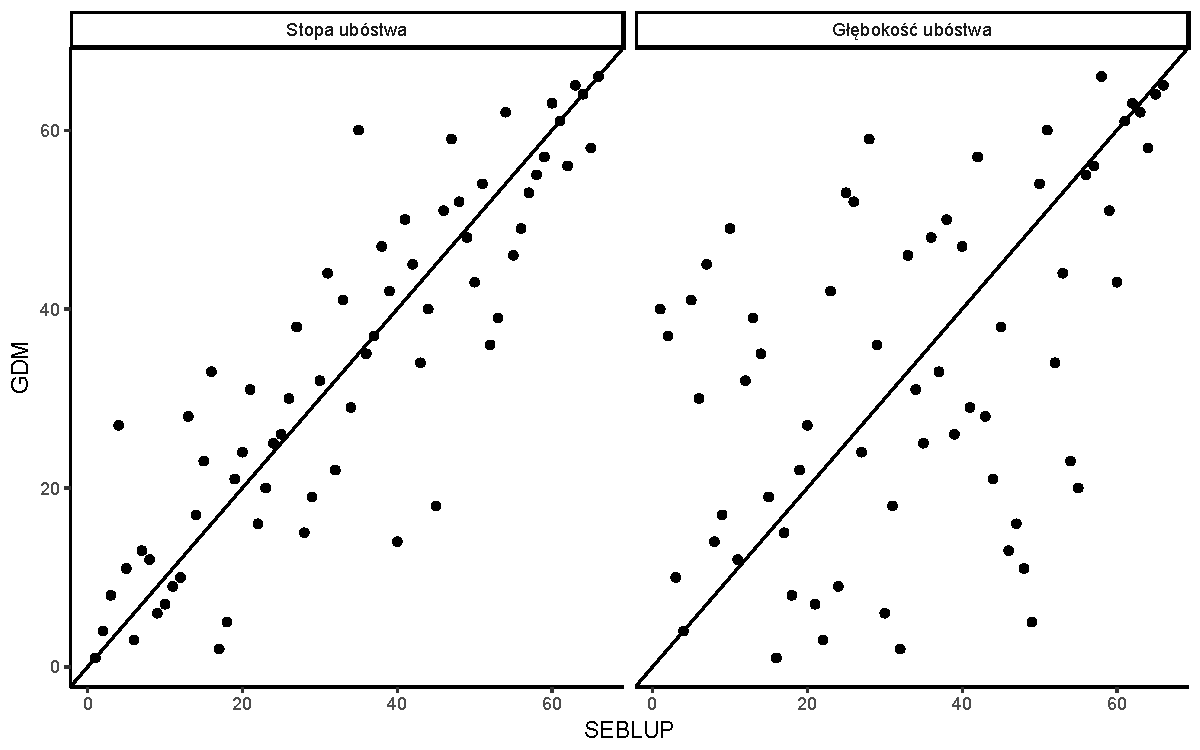
\includegraphics[width=\textwidth]{05_wykresy/podreg_gdm-1.pdf}\\
\small{Źródło: opracowanie własne na podstawie EU-SILC 2011 oraz BDL.}
\label{fig:podreg-gdm}
\end{figure}

W przypadku stopy ubóstwa te same miejsca w rankingu bez względu na zastosowaną metodę zajęły 4 podregiony --- m. Warszawa (1), podregion krakowski (37), nowosądecki (61) i puławski (64). Największy spadek w rankingu w odniesieniu do estymacji pośredniej zanotowano dla podregionu elbląskiego --- 35 miejsce według estymatora SEBLUP i 60 według miary GDM oraz miasta Kraków z 4 lokaty na 27. Z kolei największą poprawę zaobserwowano dla podregionu bytomskiego --- 35 lokata na podstawie oszacowania pośredniego i 18 miejsce na podstawie miary GDM. Drugim podregionem o równie dużej zmianie w klasyfikacji był podregion koszaliński (z 40 pozycji na 14).

Pogrupowanie obserwowanych różnic w rankingach w grupy o szerokości 10 pozycji pokazuje, że dla stopy ubóstwa w 78,8\% różnice te nie były większe niż 10 miejsc. W przedziale $(10;20]$ odnotowano 10 podregionów, natomiast zidentyfikowano tylko cztery podregiony o największym odchyleniu. W przypadku głębokości ubóstwa frakcje podregionów w poszczególnych przedziałach różnią się od tych dla zasięgu ubóstwa. W pierwszym przedziale znalazło się 45,5\% wszystkich podregionów, a w drugim 24,2\%. Pozostałe 20 podregionów charakteryzuje się różnicami przekraczającymi 20 miejsc.

% Swoje miejsca w rankingu dla głębokości ubóstwa zachowały podregiony poznański (4) oraz bialski (61). 

\subsection{Poziom powiatów}

Na poziomie powiatów ranking według poziomu ubóstwa utworzono na podstawie rezultatów otrzymanych metodą EB. Z racji tego, że dane wejściowe do tego podejścia były mierzono na poziomie gospodarstw domowych, dokonano agregacji zmiennych użytych w modelu do poziomu powiatów. Podstawą obliczeń były następujące cechy:

\begin{itemize}
\item odsetek mężczyzn w powiecie (S),
\item odsetek osób w wieku 30-44 w powiecie (S),
\item odsetek osób w wieku 65 lat i więcej w powiecie (D),
\item odsetek osób bezrobotnych w powiecie (D),
\item odsetek osób niepełnosprawnych w powiecie (D),
\item odsetek osób z wykształceniem podstawowym w powiecie (D),
\item odsetek osób z wykształceniem wyższym w powiecie (S),
\item wskaźnik obciążenia demograficznego dzieci w powiecie (D),
\item odsetek gospodarstw posiadających 1 pokój (D)
\item odsetek gospodarstw posiadających 3 pokoje i więcej (S),
\item odsetek osób zamieszkałych na wsi lub w mieście do 20 tys. osób (D),
\item stopa bezrobocia rejestrowanego (D),
\item odsetek osób zatrudnionych w rolnictwie (D),
\item wypłacone świadczenie społeczne na 1000 zatrudnionych osób (D).
\end{itemize}

Dla tak zdefiniowanego zestawu zmiennych diagnostycznych wyznaczono miarę odległości GDM oraz odległość euklidesową. Współczynnik korelacji rang Spearmana pomiędzy miarą GDM a pośrednimi oszacowaniami stopy ubóstwa był wysoki i wynosił $r_S=0,7423$. Uwzględnienie odległości euklidesowej spowodowało spadek tego współczynnika do poziomu $r_S=0,6999$. Zależność pomiędzy syntetyczną miarą rozwoju a oszacowaniami bezpośrednimi była słaba --- $r_S=0,3470$ dla miary GDM i $r_S=0,3472$ dla odległości Euklidesa. Korelacje dla wskaźnika głębokości ubóstwa były na bardzo zbliżonym poziomie.

Na rysunku \ref{fig:jedn-gdm} przedstawiono porównanie rankingu utworzonego na podstawie metody EB i~miary GDM.

\begin{figure}[ht]
\caption{Porównanie rankingów uzyskanych na podstawie estymacji pośredniej oraz miary GDM na poziomie powiatów}
\centering
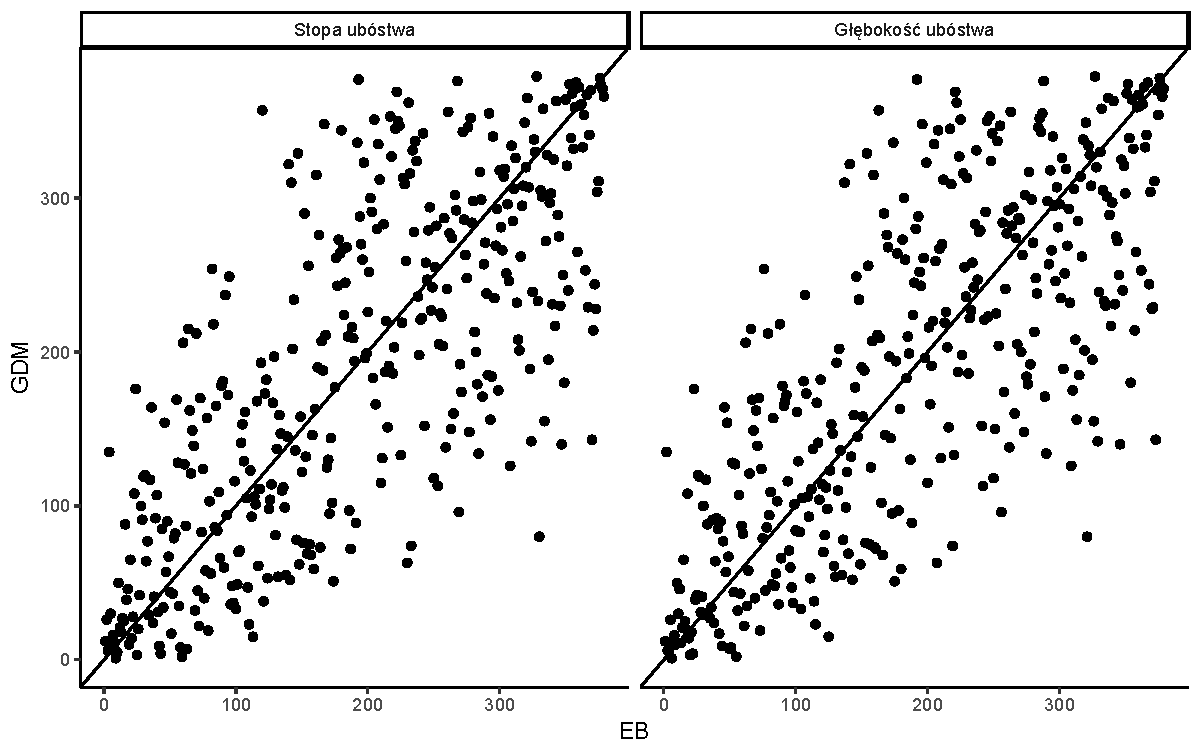
\includegraphics[width=\textwidth]{05_wykresy/jedn_gdm-1.pdf}\\
\small{Źródło: opracowanie własne na podstawie EU-SILC 2011, NSP 2011 oraz BDL.}
\label{fig:jedn-gdm}
\end{figure}

Powiaty na początku i końcu rankingu grupują się wokół prostej $y=x$, co pozwala stwierdzić, że dla tych jednostek nie występują znaczne przesunięcia. Niemniej tylko w przypadku dwóch powiatów dla stopy ubóstwa miejsca w obu rankingach pokrywają się. Są to powiaty brodnicki i pińczowski. Także dla głębokości ubóstwa z taką sytuacją mamy do czynienia tylko w dwóch jednostkach --- powiatach zgierskim i lipnowskim. Na uwagę zasługuje zmiana w klasyfikacji miasta Sopot. Powiat zajmujący 4 miejsce według poziomu zasięgu ubóstwa oraz 2 miejsce pod względem głębokości ubóstwa zajmuje 135 miejsce na podstawie rankingu GDM. 

Pogrupowanie różnic pomiędzy pozycją w rankingu według wartości wskaźnika ubóstwa oraz miary GDM w przedziały o szerokości 20 jednostek umożliwia ocenę skali zmian. W przypadku stopy ubóstwa różnica w obrębie 20 pozycji dotyczyła 100 powiatów, które stanowią 26,4\% wszystkich analizowanych jednostek. W kolejnych klasach obserwacji jest coraz mniej --- w przedziale różnic $(20;40]$ znalazło się już 19,5\% powiatów, a w kolejnym 10,8\%. Wzrost obserwowany jest dopiero dla przedziału 100 i więcej --- 20,1\% liczby powiatów. Bardzo zbliżony rozkład różnic pomiędzy pozycjami w rankingach obserwowany jest dla wskaźnika głębokości ubóstwa. 

\section{Identyfikacja i opis enklaw ubóstwa}

Na podstawie analizy przeprowadzonej w pierwszej części rozdziału jako oszacowania wskaźników ubóstwa wybrano oceny parametrów otrzymane na podstawie estymatora SEBLUP dla poziomu podregionów oraz estymatora EB dla poziomu powiatów. Opierając się na wartościach tych oszacowań utworzono kartogramy, które stały się podstawą do przeprowadzenia analizy terytorialnego zróżnicowania ubóstwa. Na rysunkach przedstawione są oszacowania stopy oraz głębokości ubóstwa w ujęciu przestrzennym.

\subsection{Poziom podregionów}

Rysunek \ref{fig:fh_nts3_hcr_pgi_4} przedstawia wartości stopy oraz głębokości ubóstwa w układzie 66 podregionów. Wartości wskaźników ubóstwa zostały pogrupowane w 4 przedziały klasowe.

\begin{figure}[ht]
\caption{Terytorialne zróżnicowanie stopy oraz głębokości ubóstwa w przekroju podregionów w 2011 roku}
\centering
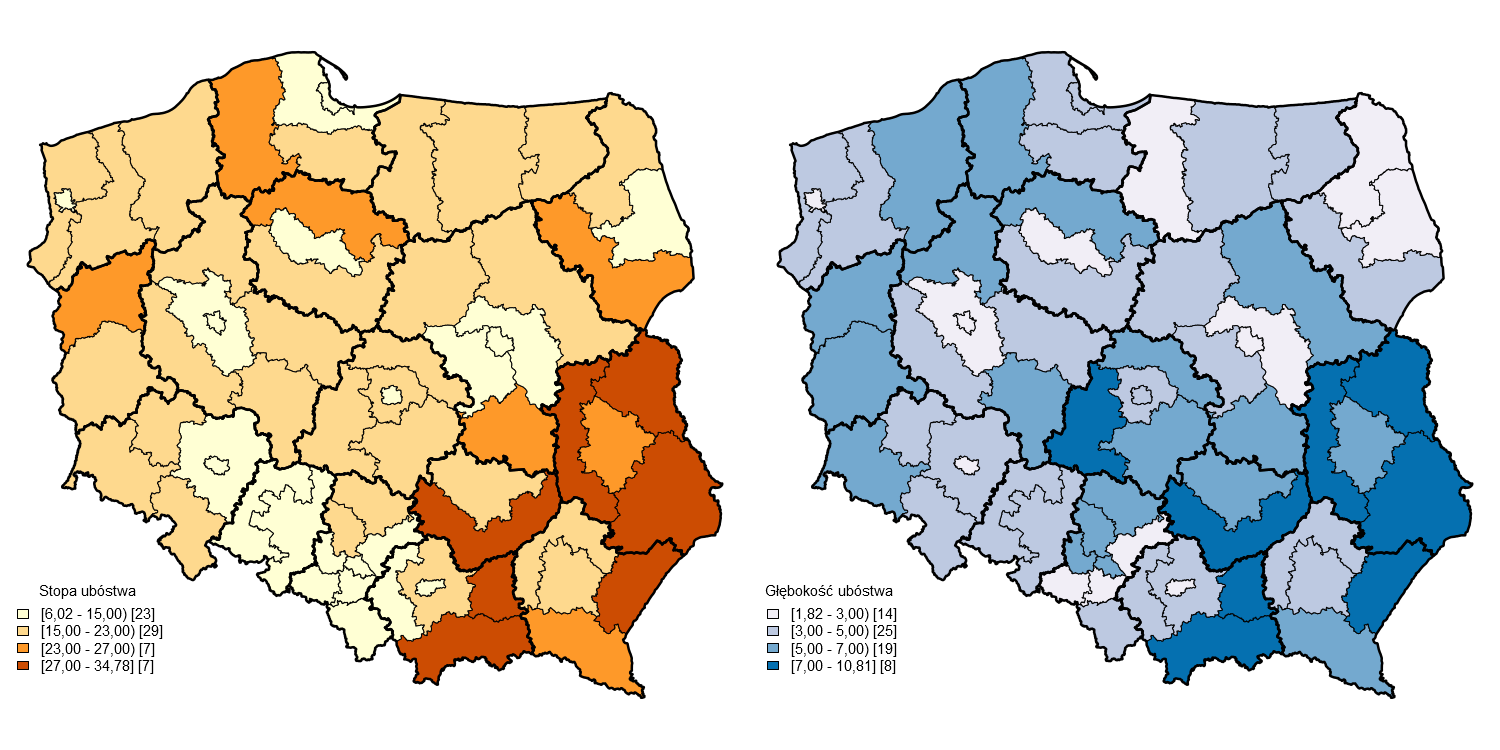
\includegraphics[width=\textwidth]{05_wykresy/fh_nts3_hcr_pgi_4.png}\\
\small{Źródło: opracowanie własne na podstawie EU-SILC 2011 oraz BDL.}
\label{fig:fh_nts3_hcr_pgi_4}
\end{figure}

Najwyższe wartości stopy ubóstwa obserwowane są w południowo-wschodniej części Polski. Są to podregiony: bialski, tarnowski, puławski, chełmsko-zamojski, sandomiersko-jędrzejowski, nowosądecki oraz przemyski. Te podregiony należą do tzw. Polski ,,B'', której w przeszłości domeną rozwoju było rolnictwo. Program Operacyjny Rozwój Polski Wschodniej realizowany ze środków UE w latach 2007--2013 miał na celu wyrównanie istniejących różnic. Z kolei najniższy poziom niedostatku obserwowany jest w podregionach, które równocześnie są miastami na prawach powiatu --- m. Warszawa, m. Wrocław, m. Poznań oraz m. Kraków. Kolejne miejsca rankingu zajmują podregiony, które częściowo tworzą konurbację górnośląską czyli podregion sosnowiecki, rybnicki, tyski oraz bielski. Wyraźnie widoczny jest wpływ dużych miast na poziom ubóstwa w ich sąsiedztwie. Przykładem może tu być m. Poznań oraz podregion poznański, m. Wrocław oraz podregion wrocławski czy podregion trójmiejski i gdański. Podregiony, które zawierają ważne ośrodki miejskie również charakteryzują się niższą stopą ubóstwa --- podregion bydgosko-toruński, podregion rzeszowski tudzież podregion białostocki.

W przypadku drugiej analizowanej cechy --- głębokości ubóstwa, najmniejsza luka dochodowa wśród osób żyjących poniżej linii ubóstwa obserwowana jest w podregionach m. Warszawa, m.~Wrocław, m. Poznań, białostockim oraz poznańskim. Największe ubóstwo ubogich występuję w~tych samych podregionach, w których zidentyfikowano także najwyższe wartości stopy ubóstwa. Podregion suwalski jest przykładem obszaru, który charakteryzuje się dosyć wysoką stopą ubóstwa --- 19,9\%, a równocześnie niskim poziomem ubóstwa osób ubogich --- 2,6\%. Na rysunku \ref{fig:fh_nts3_hcr_pgi_4} wyróżnia się podregion sieradzki w województwie łódzkim, który znajduje się w przedziale klasowym o najwyższej głębokości ubóstwa, natomiast wartość stopy ubóstwa jest na poziomie całego województwa. Jest to przykład niedoskonałości narzędzia prezentacji, jakim jest mapa o sztywno ustalonych przedziałach klasowych. W podregionie sieradzkim stopa ubóstwa wynosi 22,4\% czyli bliżej górnej granicy przedziału klasowego, a głębokość ubóstwa 7\% czyli na granicy przedziału klasowego.

Uzupełnieniem analizy była klasyfikacja wartości wskaźników ubóstwa do 3 grup metodą k-średnich. W tym celu zastosowano funkcję \textit{classIntervals} z pakietu \textit{classInt} \citep{classint2015}.

\begin{figure}[ht]
\caption{Klasyfikacja stopy oraz głębokości ubóstwa w przekroju podregionów w 2011 roku}
\centering
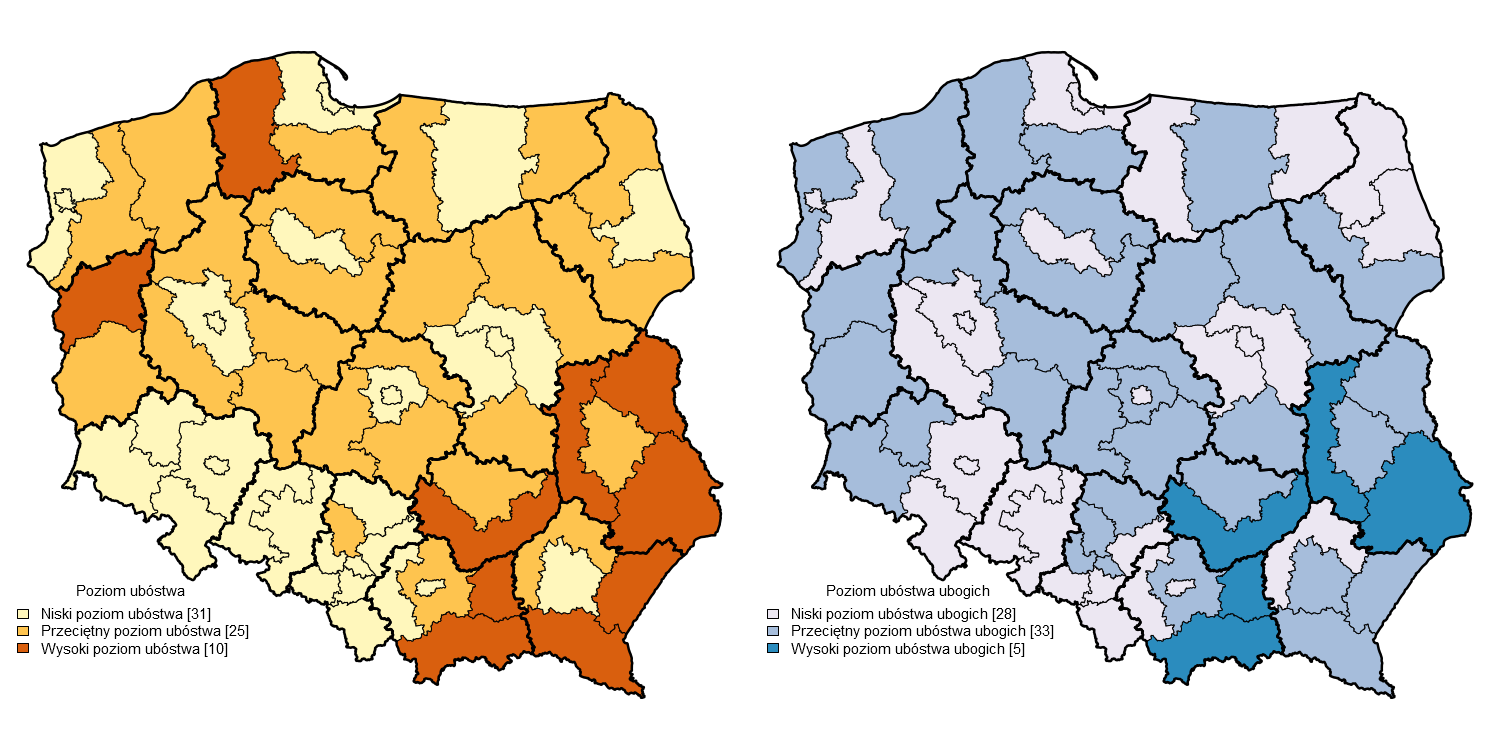
\includegraphics[width=\textwidth]{05_wykresy/fh_nts3_hcr_pgi_k3.png}\\
\small{Źródło: opracowanie własne na podstawie EU-SILC 2011 oraz BDL.}
\label{fig:fh_nts3_hcr_pgi_k3}
\end{figure}

Przeprowadzona klasyfikacja pozwoliła na wyróżnienie enklaw charakteryzujących się występowaniem niskiego, przeciętnego oraz wysokiego poziomu ubóstwa oraz ubóstwa osób ubogich. Podregionów charakteryzujących się niskim poziomem ubóstwa jest 31. W tej klasie znajdują się podregiony o wartościach stopy ubóstwa nieprzekraczającej 16,6\%. Do tej grupy zaklasyfikowano podregiony będące miastami oraz zawierające duże ośrodki miejskie. Cały obszar Śląska został także zaklasyfikowany do tej grupy za wyjątkiem podregionu bytowskiego. Wysoki poziom ubóstwa występuje w podregionach Polski południowo-wschodniej --- w województwach małopolskim, podkarpackim, lubelskim, świętokrzyskim. Ponadto do tej grupy przynależą dwa podregiony leżące w północnej części kraju --- słupski i gorzowski. Wartością, która determinowała zaklasyfikowanie do klasy o wysokim poziomie ubóstwa było oszacowanie stopy ubóstwa powyżej 24,8\%. 

Podobnie jak w przypadku stopy ubóstwa niski poziom ubóstwa ubogich odnotowuje się głównie w ośrodkach miejskich. Pierwszą grupę stanowią podregiony, w których oszacowane głębokości ubóstwa nie przekraczało 4,2\%. Do grupy obszarów o wysokim poziomie ubóstwa osób ubogich zaklasyfikowano 5 podregionów znajdujących się w południowo-wschodniej części kraju. Głębokość ubóstwa w tych podregionach była wyższa od 7,6\%.

Uzyskane wyniki przeanalizowano także pod katem spójności przestrzennej. W tym celu wyznaczono statystykę Morana I dla stopy i głębokości ubóstwa wykorzystując macierz sąsiedztwa podregionów. Obliczone wartości statystyki wykazały istnienie dodatniej autokorelacji oszacowań. Wartość statystyki dla stopy ubóstwa była równa 0,47, a dla głębokości ubóstwa 0,37 i była istotna statystycznie. 

%Obliczenia przeprowadzono funkcją \textit{moran.test} z pakietu \textit{spdep} 

\subsection{Poziom powiatów}

Specyfika podziału terytorialnego Polski powoduje, że kolejny poziom estymacji charakteryzuje się prawie sześciokrotnym wzrostem liczby domen. Na rysunku \ref{fig:eb_nts4_hcr_pgi_7} przedstawiono wartości stopy i głębokości ubóstwa dla powiatów. Z racji większej liczby jednostek oraz większej rozpiętości oszacowań zastosowano 7-stopniową skalę barw. 

\begin{figure}[ht]
\caption{Terytorialne zróżnicowanie stopy oraz głębokości ubóstwa w przekroju powiatów w 2011 roku}
\centering
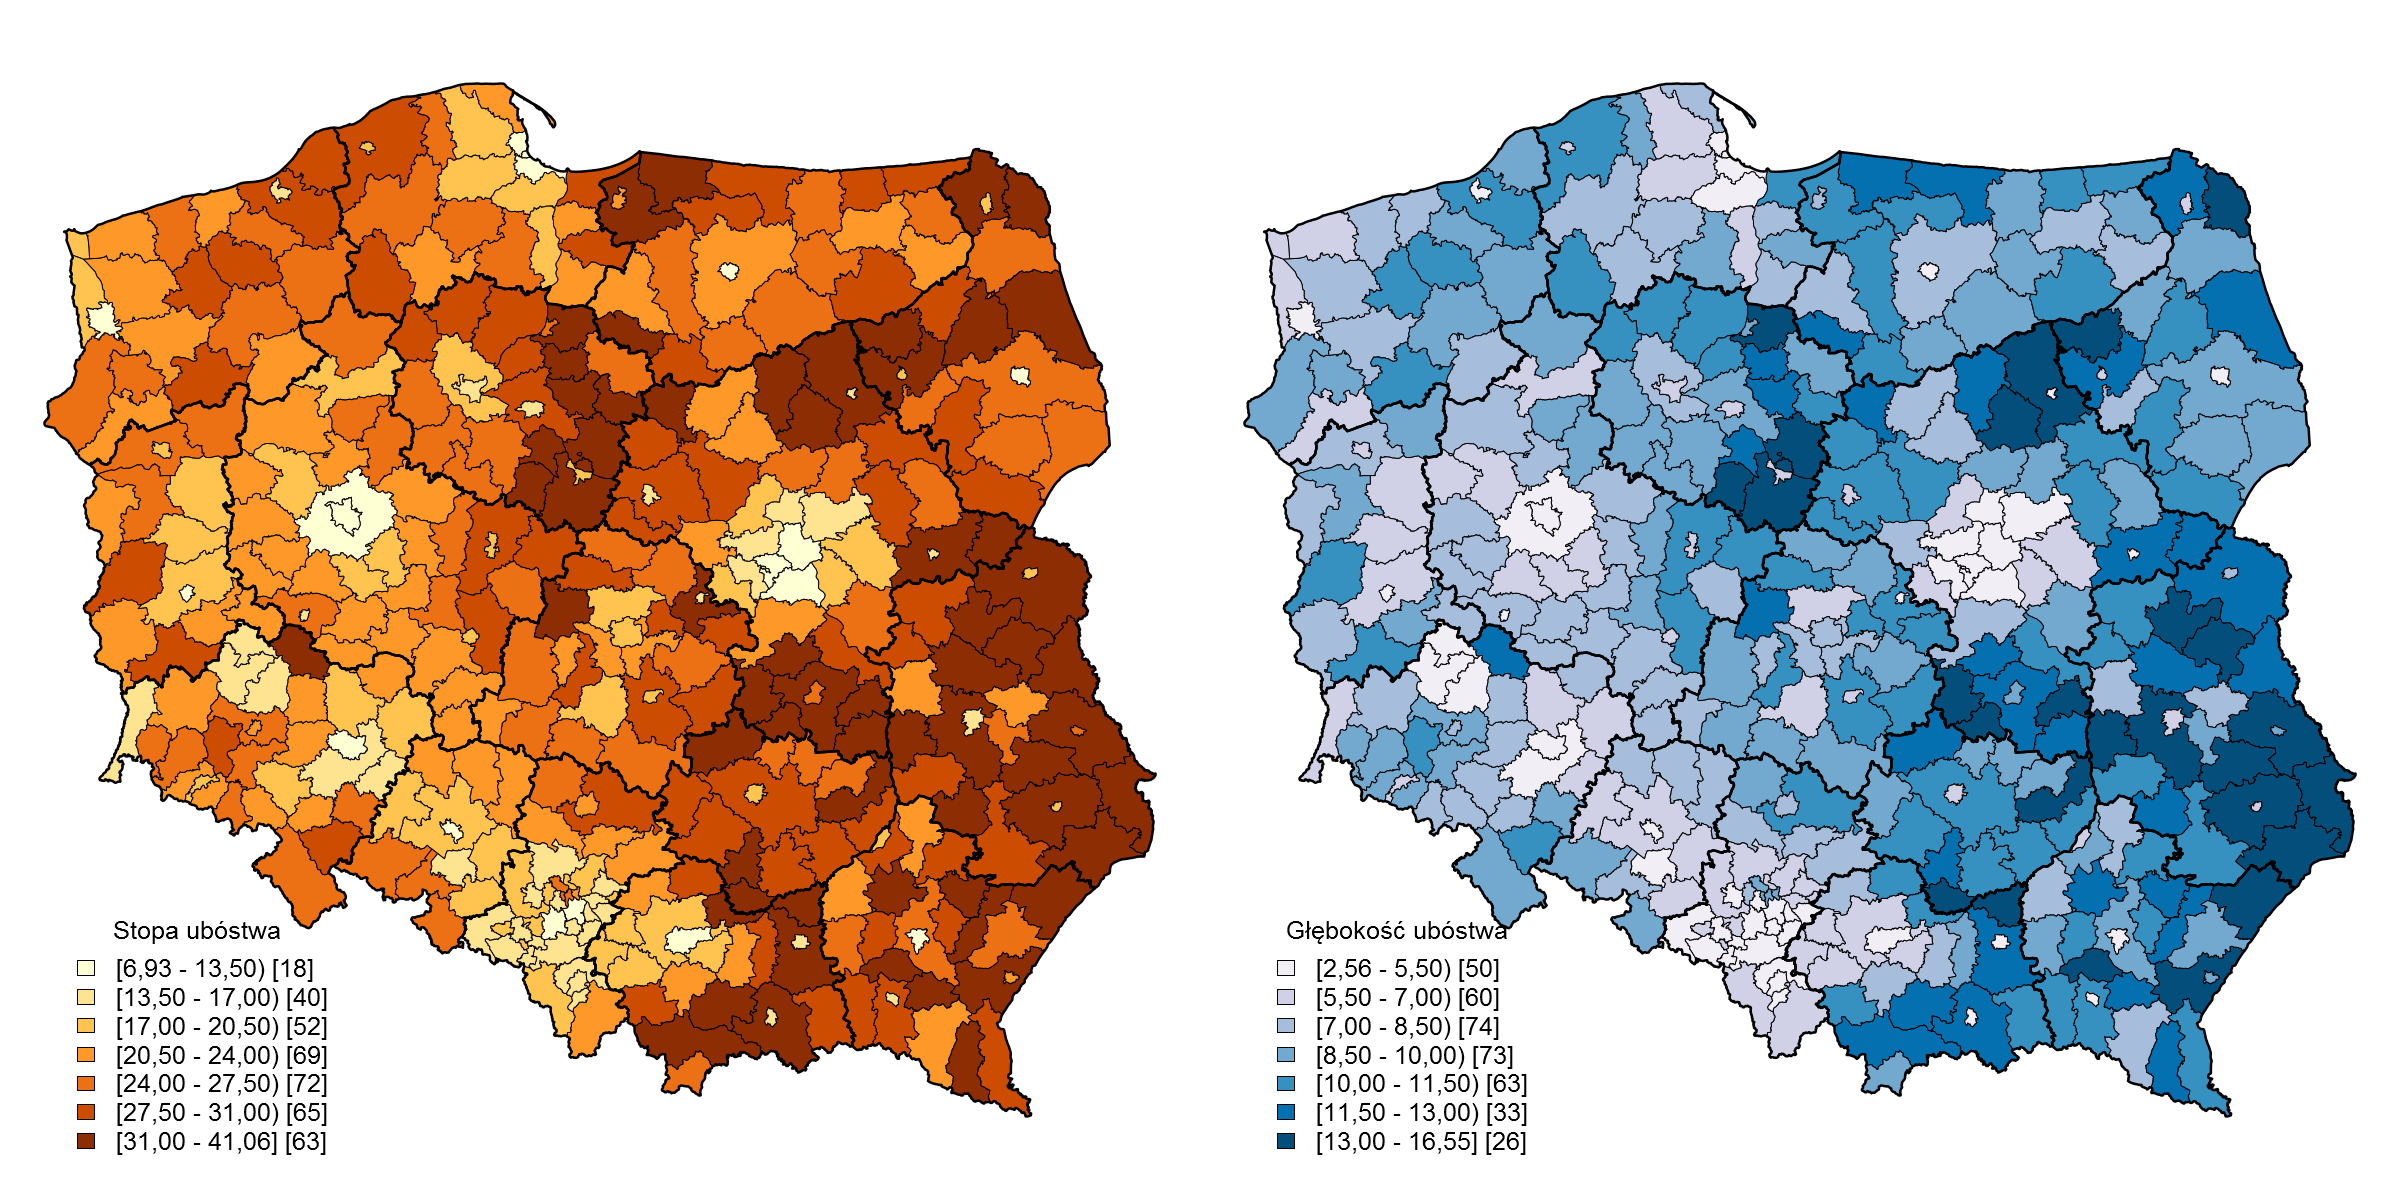
\includegraphics[width=\textwidth]{05_wykresy/eb_nts4_hcr_pgi_7.png}\\
\small{Źródło: opracowanie własne na podstawie EU-SILC 2011, NSP 2011 oraz BDL.}
\label{fig:eb_nts4_hcr_pgi_7}
\end{figure}

Najwyższe wartości stopy ubóstwa są obserwowane w powiatach znajdujących się we wschodniej części kraju oraz jednostkach znajdujących się w znacznej odległości od stolic województw. Występowaniem największego ubóstwa --- powyżej 40\% --- charakteryzuje się powiat chełmski (41,1\%) oraz hrubieszowski (40,9\%). Wśród 20 powiatów o najwyższych wartościach stopy ubóstwa znajdują się trzy powiaty położone we wschodniej części województwa kujawsko-pomorskiego, pięć powiatów województwa lubelskiego oraz jeden powiat znajdujący się w województwie małopolskim (powiat dąbrowski). Aż pięć powiatów pochodzi z województwa mazowieckiego, przy czym są to powiaty znacznie oddalone od miasta stołecznego Warszawa: ostrołęcki i makowski (znajdujące się w północnej części województwa) oraz przysuski, szydłowiecki i zwoleński (umiejscowione w południowej części województwa). Wśród tych dwudziestu jednostek po dwie pochodzą z województwa podkarpackiego, podlaskiego i świętokrzyskiego.

Najniższe wartości stopy ubóstwa to miasta na prawach powiatu oraz powiaty bezpośrednio z nimi sąsiadujące. Na pierwszym miejscu jest m. st. Warszawa (6,9\%), na drugim m. Poznań (10,9\%), a na trzecim, graniczący z Warszawą powiat pruszkowski (11,2\%). Dalsze pozycje rankingu zajmują miasta na prawach powiatu: m. Gdynia, m. Sopot (po 11,7\%), m. Opole, m. Rzeszów, m. Olsztyn (po 12,8\%). Wśród 20 powiatów o najniższej stopie ubóstwa znajdują się wyłącznie miasta na prawach powiatu oraz jednostki bezpośrednio graniczące z tymi powiatami.

W przypadku wartości luki dochodowej obserwowana jest wysoka korelacji tej cechy ze stopą ubóstwa ($r=0,99$). Najmniejsze ubóstwo wśród osób ubogich obserwowane jest w Warszawie (2,6\%) Na kolejnych miejscach znajdują się: powiat pruszkowski i miasto Sopot (po 3,8\%) oraz powiat poznański i miasto Poznań (po 3,9\%). Najwyższe oszacowania wskaźnika głębokości ubóstwa odnotowano w tych samych powiatach, w których występowała wysoka stopa ubóstwa. 

Na podstawie wartości wskaźników ubóstwa, na poziomie powiatów także dokonano klasyfikacji, tym razem tworząc 5 grup poziomu ubóstwa. Wyniki klasyfikacji przedstawione są na rysunku \ref{fig:eb_nts4_hcr_pgi_k5}.

\begin{figure}[ht]
\caption{Klasyfikacja stopy oraz głębokości ubóstwa w przekroju powiatów w 2011 roku}
\centering
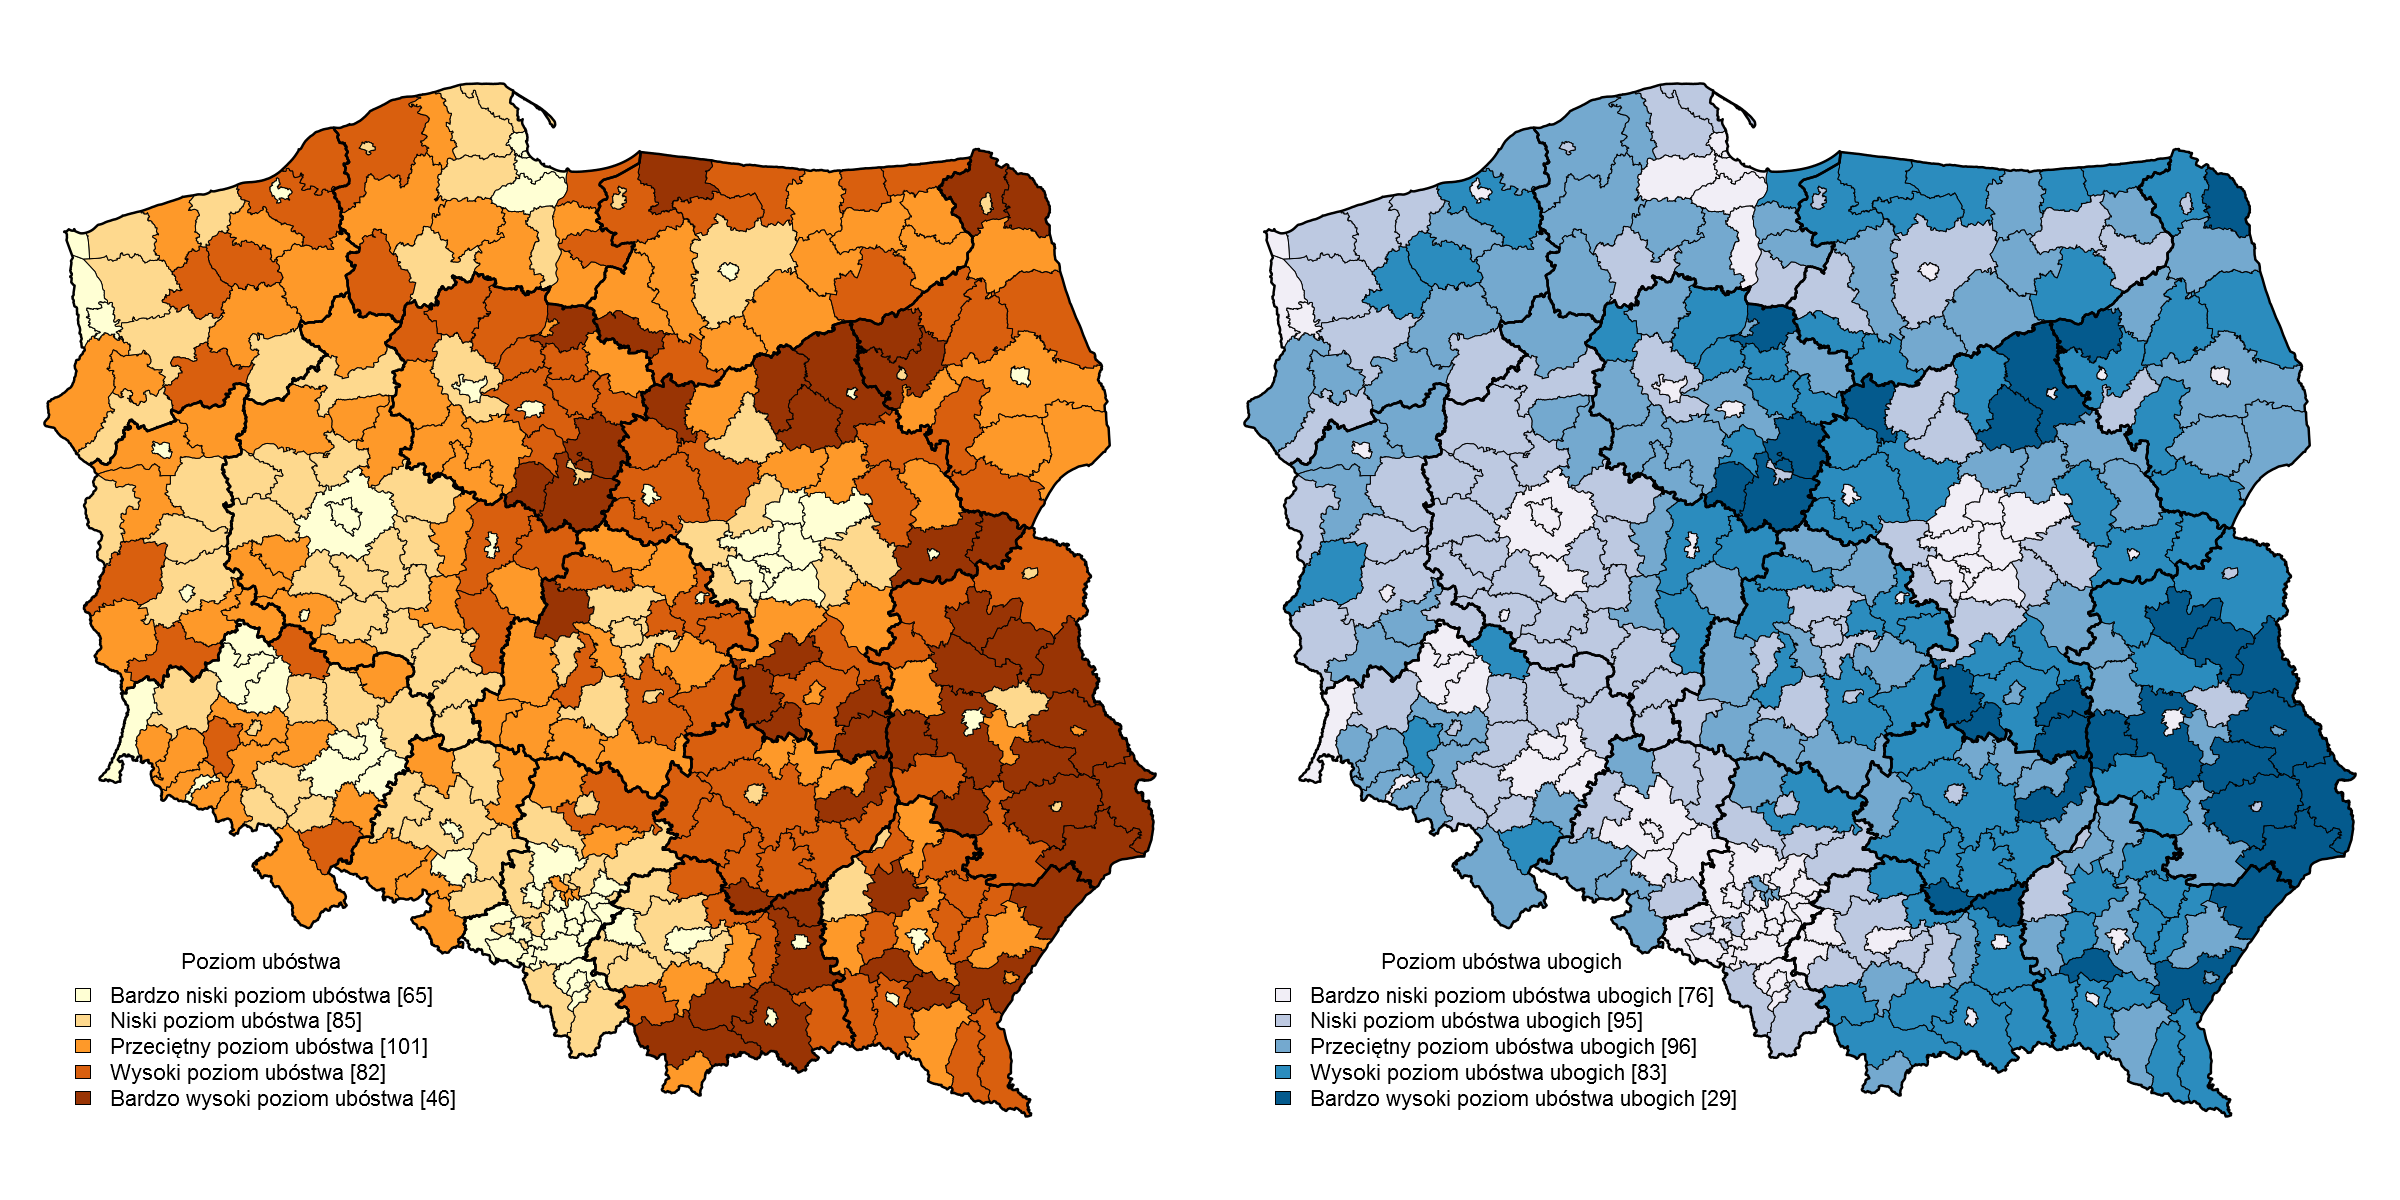
\includegraphics[width=\textwidth]{05_wykresy/eb_nts4_hcr_pgi_k5.png}\\
\small{Źródło: opracowanie własne na podstawie EU-SILC 2011, NSP 2011 oraz BDL.}
\label{fig:eb_nts4_hcr_pgi_k5}
\end{figure}

W przypadku powiatów wyróżniono 5 poziomów ubóstwa. Do grupy o bardzo niskim poziomie ubóstwa zaklasyfikowano 65 powiatów. Tyle wynosi liczba miast na prawach powiatu w Polsce, ale w tej grupy nie znalazły się wszystkie z nich. Granicą przynależności do tych powiatów była wartość wskaźnika stopy ubóstwa poniżej 17,4\%. Najwięcej powiatów znalazło się w grupie cechującej się przeciętnym poziomem ubóstwa --- 27\% wszystkich powiatów o wartościach zasięgu ubóstwa z przedziału $[22,7\% -- 27,4\%]$. Do klasy powiatów o bardzo wysokim poziomie ubóstwa (powyżej 32,4\%) włączono 46 jednostek znajdujących się przede wszystkim we wschodniej części Polski. Łącznie w kategoriach zawierających powiaty o bardzo niskim oraz niskim poziomie ubóstwa znalazło się 150 jednostek administracyjnych, a w grupach wysokiego i bardzo wysokiego poziomu ubóstwa 128 powiatów. 

Analiza klas wyłonionych dla wskaźnika głębokości ubóstwa wskazuje, że ubóstwo osób ubogich nie jest bardzo wysokie. Powiatów o bardzo niskim poziomie ubóstwa ubogich jest 76 --- o 11 więcej, w porównaniu do tej samej klasy opisującej stopę ubóstwa. W tej grupie znalazły się powiaty charakteryzujące się głębokością ubóstwa mniejszą niż 6,2\%. Przeciętna wartość luki dochodowej zawiera się w przedziale $[8,2\% -- 10,2\%]$ i jest charakterystyczna dla 96 powiatów. Jednostek o bardzo wysokim ubóstwie osób żyjących poniżej granicy niedostatku jest zaledwie 29. W tej grupie wskaźnik głębokości ubóstwa przekracza 12,6\%. Także w przypadku tego wskaźnika obserwowana jest wyraźna przewaga liczby powiatów w grupach poniżej przeciętnych wartości (171 domen) w porównaniu do liczby powiatów o wysokim i bardzo wysokim poziomie ubóstwa osób ubogich (112).

Na podstawie wartości wskaźników ubóstwa oszacowanych na szczeblu powiatowym oraz macierzy sąsiedztwa obliczono także statystykę Morana I. Podobnie jak w przypadku poziomu podregionów, także na tym poziomie terytorialnym odnotowano istnienie dodatniej korelacji przestrzennej --- statystyka wynosiła odpowiednio 0,45 dla stopy i 0,47 dla głębokości ubóstwa. 

\section{Podsumowanie}

Celem działań przeprowadzonych w rozdziale piątym była analiza wskaźników ubóstwa oszacowanych z wykorzystaniem metod statystyki małych obszarów, która uwzględniała zarówno ocenę dotyczącą wykorzystanych metod, jak i wymiar przestrzenny. Dane statystyczne, które zawierałyby informację o stopie oraz głębokości ubóstwa w populacji nie są nigdzie publikowane, w~związku z czym weryfikacja uzyskanych szacunków pośrednich bazowała na porównaniu z cechami mogącymi przybliżyć dane zjawisko, tzw. \textit{zmiennymi proxy}. Po gruntownej analizie dostępnych źródeł danych zdecydowano się na odwołanie się do informacji pochodzących z rejestrów administracyjnych, które dotyczyły bezrobocia rejestrowanego oraz korzystania z pomocy społecznej. Wykazano, że oszacowania pośrednie są silniej skorelowane ze wskaźnikami bezrobocia długotrwałego oraz korzystania z pomocy społecznej, aniżeli te, oszacowane z zastosowaniem estymatora bezpośredniego. 

Jako narzędzie oceny oszacowań pośrednich zaproponowano metody wielowymiarowej analizy statystycznej, a dokładnie syntetyczny miernik rozwoju. Wyznaczenie rankingu dla podregionów i powiatów bazowało na zmiennych niezależnych zidentyfikowanych jako zmienne pomocnicze w~modelach obszarowych oraz jednostkowych wypracowanych w rozdziale 4. Na podstawie tak określonego zestawu cech diagnostycznych wyznaczono odległość euklidesową oraz GDM od obiektu wzorcowego. Porównanie współczynników korelacji rang Spearmana oszacowań pośrednich wskaźników ubóstwa oraz syntetycznych mierników rozwoju wykazało istnienie silnej dodatniej zależności pomiędzy rankingiem uzyskanym na podstawie wartości zasięgu ubóstwa, a miarą odległości GDM. Zależność ta była słabsza w przypadku zastosowania euklidesowej miary odległości. Wyniki przeprowadzonej analizy świadczą o tym, że miara odległości GDM może stanowić narzędzie merytorycznej oceny oszacowań wskaźników ubóstwa oraz może służyć do wykrywania wartości nietypowych.

W ostatniej części rozdziału dokonano przestrzennej oceny wskaźników ubóstwa oszacowanych z wykorzystaniem metod estymacji pośredniej. Zidentyfikowano obszary, znajdujące się głównie we wschodniej części Polski, charakteryzujące się wysokim poziomem ubóstwa. Jednostkami, które cechują się niskim ubóstwem są przede wszystkim duże miasta oraz powiaty je okalające. Wraz ze wzrostem odległości do najbliższego dużego ośrodka miejskiego rośnie także poziom niedostatku. Obserwuje się także niskie ubóstwo na terenie praktycznie całego Śląska, co może być uzasadnione istnieniem autostrady A4 łączącej wszystkie większe ośrodki miejskie na tym terenie. Pomiędzy oszacowaniami wskaźników ubóstwa istnieje umiarkowana dodatnia autokorelacja przestrzenna świadcząca o podobieństwie wartości sąsiadujących.